\section{Output stages}
\subsection{Introduction}
\subsubsection*{Goal}
Due to the maximum current limits of the op amps, they cannot be used to drive loads (speakers) directly. A power amplifier is
needed to preserve the same signal waveform, but with higher current and power. A good power amplifier should have:
\begin{itemize}
	\item support for large signal operation (10-20 V)
	\item low output impedance (to drive low impedance loads with high efficiency)
	\item low harmonic distortion (to preserve the signal waveform)
\end{itemize}

\subsubsection*{Power amplifiers classes}
\begin{itemize}
	\item class A: the output stage is always on, even without input signal
	\item class B: the output stage is on only for half of the input signal period
	\item class AB: the output stage is on for more than half of the input signal period
	\item class C: the output stage is on for less than half of the input signal period
\end{itemize}

\subsubsection*{THD - Total Harmonic Distortion}
The total harmonic distortion (THD) is a measure of the quality of the output signal. It is defined as the ratio of the RMS power
of the entire harmonic content (excluding the fundamental frequency) of the output signal to the RMS power of the fundamental
frequency.
\[THD = \frac{\sqrt{{V_2}^2 + {V_3}^2 + {V_4}^2 + \cdots}}{V_1} = \frac{\sqrt{\sum_{i \geq 2} {V_i}^2}}{V_1}\]

\subsection{Class A - Emitter follower}
\subsubsection*{Circuit description}
The simplest class A output stage is the emitter follower, which is a BJT transistor in which the input signal is applied to
the base and the output is taken from the emitter. The collector is connected to the supply voltage. This configuration is
called ``emitter follower'' because the output voltage in the emitter follows the input voltage at the base, with a fixed
voltage drop \(V_{BE}\). The transistor acts also as a current amplifier to drive the load with appropriate power.
\[V_{out} = V_{in} - V_{BE} \qquad\qquad I_E = \beta I_B\]

To ensure that the transistor is always on, there must be a bias current flowing from the emitter, even without input signal.
This can be achieved by using a current generator connected between the emitter and ground. The generator current \(I_{gen}\)
must be higher than the maximum current \(I_{L,max}\) that can be delivered to the load, to ensure that \(I_E\) current is
always positive.
\[I_{E} = I_{gen} + I_L > 0 \quad \rightarrow \quad I_{gen} > \left|I_L\right|\]

\begin{center}
	\begin{minipage}{0.5\textwidth}
		\centering\begin{circuitikz}[american, scale=0.8, transform shape]
			\node[npn] (Q1) at (0,0) {};
			\node[right] at (Q1) {$Q_1$};
			\draw (Q1.B) to[short, -o] ++(-0.5,0) node[left] {$V_{in}$};
			\draw (Q1.C) to[short, -o] ++(0,0) node[above] {$+V_{CC}$};
			\draw (Q1.E) to[short, i=\(I_{E}\)] ++(0,-0.5) coordinate (outSplit);
			\draw (outSplit) -- ++(0.5,0) to[short, -o, i_=\(I_L\)] ++(1,0) node[right] {$V_{out}$}
				to[R, l=\(R_L\)] ++(0, -2) ++(0,0.4)node[ground] {};
			\draw (outSplit) to[isource, l_=$I_{gen}$, -o] ++(0,-1.5) node[below] {$-V_{CC}$};
	
			\node [xshift=-0.1cm, yshift=-0.2cm] at (Q1.B) (vplus) {$+$};
			\node [xshift=-0.3cm, yshift=-0.3cm] at (Q1.E) (vminus) {$-$};
			\draw (vminus) to node[midway, fill=white, inner sep=3pt] {$V_{BE}$} (vplus);
		\end{circuitikz}
	\end{minipage}
\end{center}

\subsubsection*{With diode to bias transistor}
It is possible implement the ideal current generator by using a diode with a fixed voltage drop \(V_D\) to impose a fixed voltage
drop \(V_{BE2} = V_D\) across the transistor \(Q_2\) that generates the constant current \(I_{gen}\).

The problem is that small variations on the voltage \(V_D\) (due to component heating) are exponentially amplified in current
variations \(I_{gen}\) by the transistor \(Q_2\) and the output stage becomes unstable.

\begin{center}
	\begin{minipage}{0.4\textwidth}
		\centering \begin{circuitikz}[american, scale=0.8, transform shape]
			\ctikzset{diodes/scale=0.8}
			\node[npn] (Q1) at (0,0) {\(Q_1\)};
			\draw (Q1.B) to[short, -o] ++(-0.5,0) node[left] {$V_{in}$};
			\draw (Q1.C) to[short, -o] ++(0,0) node[above] {$+V_{CC}$};
			\draw (Q1.E) to[short, i=\(I_{E}\)] ++(0,-0.5) coordinate (outSplit);
			\draw (outSplit) -- ++(0.5,0) to[short, -o, i_=\(I_L\)] ++(1,0) node[right] {$V_{out}$}
				to[R, l=\(R_L\)] ++(0, -2) ++(0,0.4)node[ground] {};
			
			\node[npn, anchor=collector] at (outSplit) (Q2) {\(Q_2\)};
			\draw (Q2.E) to[short, -o, i=\(I_{gen}\)] ++(0,-0.7) node[below] {$-V_{CC}$};

			\draw (Q2.B) -- ++(-2,0) to[D, l=\(D\)] ++(0,-1.5) to[short, -o] ++(0,0) node[below] {$-V_{CC}$};
			\draw (Q2.B) -- ++(-2,0) to[R, l_=\(R\)] ++(0,1.5) to[short] ++(0,0) node[ground, yscale=-1] {};
	
			\node [xshift=-0.1cm, yshift=-0.2cm] at (Q1.B) (vplus) {$+$};
			\node [xshift=-0.3cm, yshift=-0.3cm] at (Q1.E) (vminus) {$-$};
			\draw (vminus) to node[midway, fill=white, inner sep=3pt] {$V_{BE1}$} (vplus);

			\node [xshift=-0.1cm, yshift=-0.2cm] at (Q2.B) (vplus) {$+$};
			\node [xshift=-0.3cm, yshift=-0.3cm] at (Q2.E) (vminus) {$-$};
			\draw (vminus) to node[midway, fill=white, inner sep=3pt] {$V_{BE2}$} (vplus);
		\end{circuitikz}
	\end{minipage}
	\begin{minipage}{0.45\textwidth}
		\[I_{gen} = I_{C2} = I_S \left( e^{V_{BE2} / V_T} - 1 \right)\]
	\end{minipage}
\end{center}

\subsubsection*{With current mirror transistors}
The idea is to use a current mirror to generate the bias current \(I_{gen}\) for the output stage. The current mirror is made
of two matched transistors \(Q_2\) and \(Q_3\) that share the same base voltage \(V_{BE2} = V_{BE3}\) and therefore the same
working point. The current \(I_{gen}\) is set by the resistor \(R\) and the voltage drop \(V_{BE3}\) across the transistor \(Q_3\).

The problem of this configuration is that the current mirror transistor should be matched (should come from the same silicon wafer)
and sometimes this requirement is impossible to achieve.

\begin{center}
	\begin{minipage}{0.4\textwidth}
		\centering\begin{circuitikz}[american, scale=0.8, transform shape]
			\node[npn] (Q1) at (0,0) {\(Q_1\)};
			\draw (Q1.B) to[short, -o] ++(-0.5,0) node[left] {$V_{in}$};
			\draw (Q1.C) to[short, -o] ++(0,0) node[above] {$+V_{CC}$};
			\draw (Q1.E) to[short, i=\(I_{E}\)] ++(0,-0.5) coordinate (outSplit);
			\draw (outSplit) -- ++(0.5,0) to[short, -o, i_=\(I_L\)] ++(1,0) node[right] {$V_{out}$}
				to[R, l=\(R_L\)] ++(0, -2) ++(0,0.4)node[ground] {};
			
			\node[npn, anchor=collector] at (outSplit) (Q2) {\(Q_2\)};
			\node[npn, anchor=base, xshift=-0.5cm, xscale=-1] at (Q2.B) (Q3) {};
			\node[left] at (Q3) {\(Q_3\)};
			\draw (Q3.B) -- (Q2.B);
			\draw (Q2.E) to[short, -o, i=\(I_{gen}\)] ++(0,-0.7) node[below] {$-V_{CC}$};
			\draw (Q3.E) to[short, -o, i_=\(I_{gen}\)] ++(0,-0.7) node[below] {$-V_{CC}$};

			\draw (Q3.C) -- ++(0.6,0) -- (Q3.B);
			\draw (Q3.C) to[R, l_=\(R\)] ++(-2,0) node[ground] {};
	
			\node [xshift=-0.1cm, yshift=-0.2cm] at (Q1.B) (vplus) {$+$};
			\node [xshift=-0.3cm, yshift=-0.3cm] at (Q1.E) (vminus) {$-$};
			\draw (vminus) to node[midway, fill=white, inner sep=3pt] {$V_{BE1}$} (vplus);

			\node [xshift=-0cm, yshift=-0.2cm] at (Q2.B) (vplus) {$+$};
			\node [xshift=-0.3cm, yshift=-0.3cm] at (Q2.E) (vminus) {$-$};
			\draw (vminus) to node[midway, fill=white, inner sep=3pt] {$V_{BE2}$} (vplus);

			\node [xshift=0cm, yshift=-0.2cm] at (Q3.B) (vplus) {$+$};
			\node [xshift=0.3cm, yshift=-0.3cm] at (Q3.E) (vminus) {$-$};
			\draw (vminus) to node[midway, fill=white, inner sep=3pt] {$V_{BE3}$} (vplus);
		\end{circuitikz}
	\end{minipage}
	\begin{minipage}{0.45\textwidth}
		\[I_{gen} = I_R = \frac{V_R}{R} = \frac{\left|-V_{CC}\right| - V_{BE3}}{R}\]
	\end{minipage}
\end{center}

\subsubsection*{Transfer characteristic}
The transfer characteristic of the emitter follower is a straight line with a slope of 1 and a vertical offset of \(-V_{BE1}\).
The upper limit of the output voltage is \(V_{CC} - V_{CE1sat}\) that occurs when the transistor \(Q_1\) is in saturation. The
lower limit of the output voltage is the minimum (in absolute value) between \(-V_{CC}+V_{CE2sat}\) (saturation of \(Q_2\)) and
\(-I_{gen} \cdot R_L\) (maximum load current before \(Q_1\) enters cutoff).

\begin{center}
	\begin{minipage}{0.45\textwidth}
		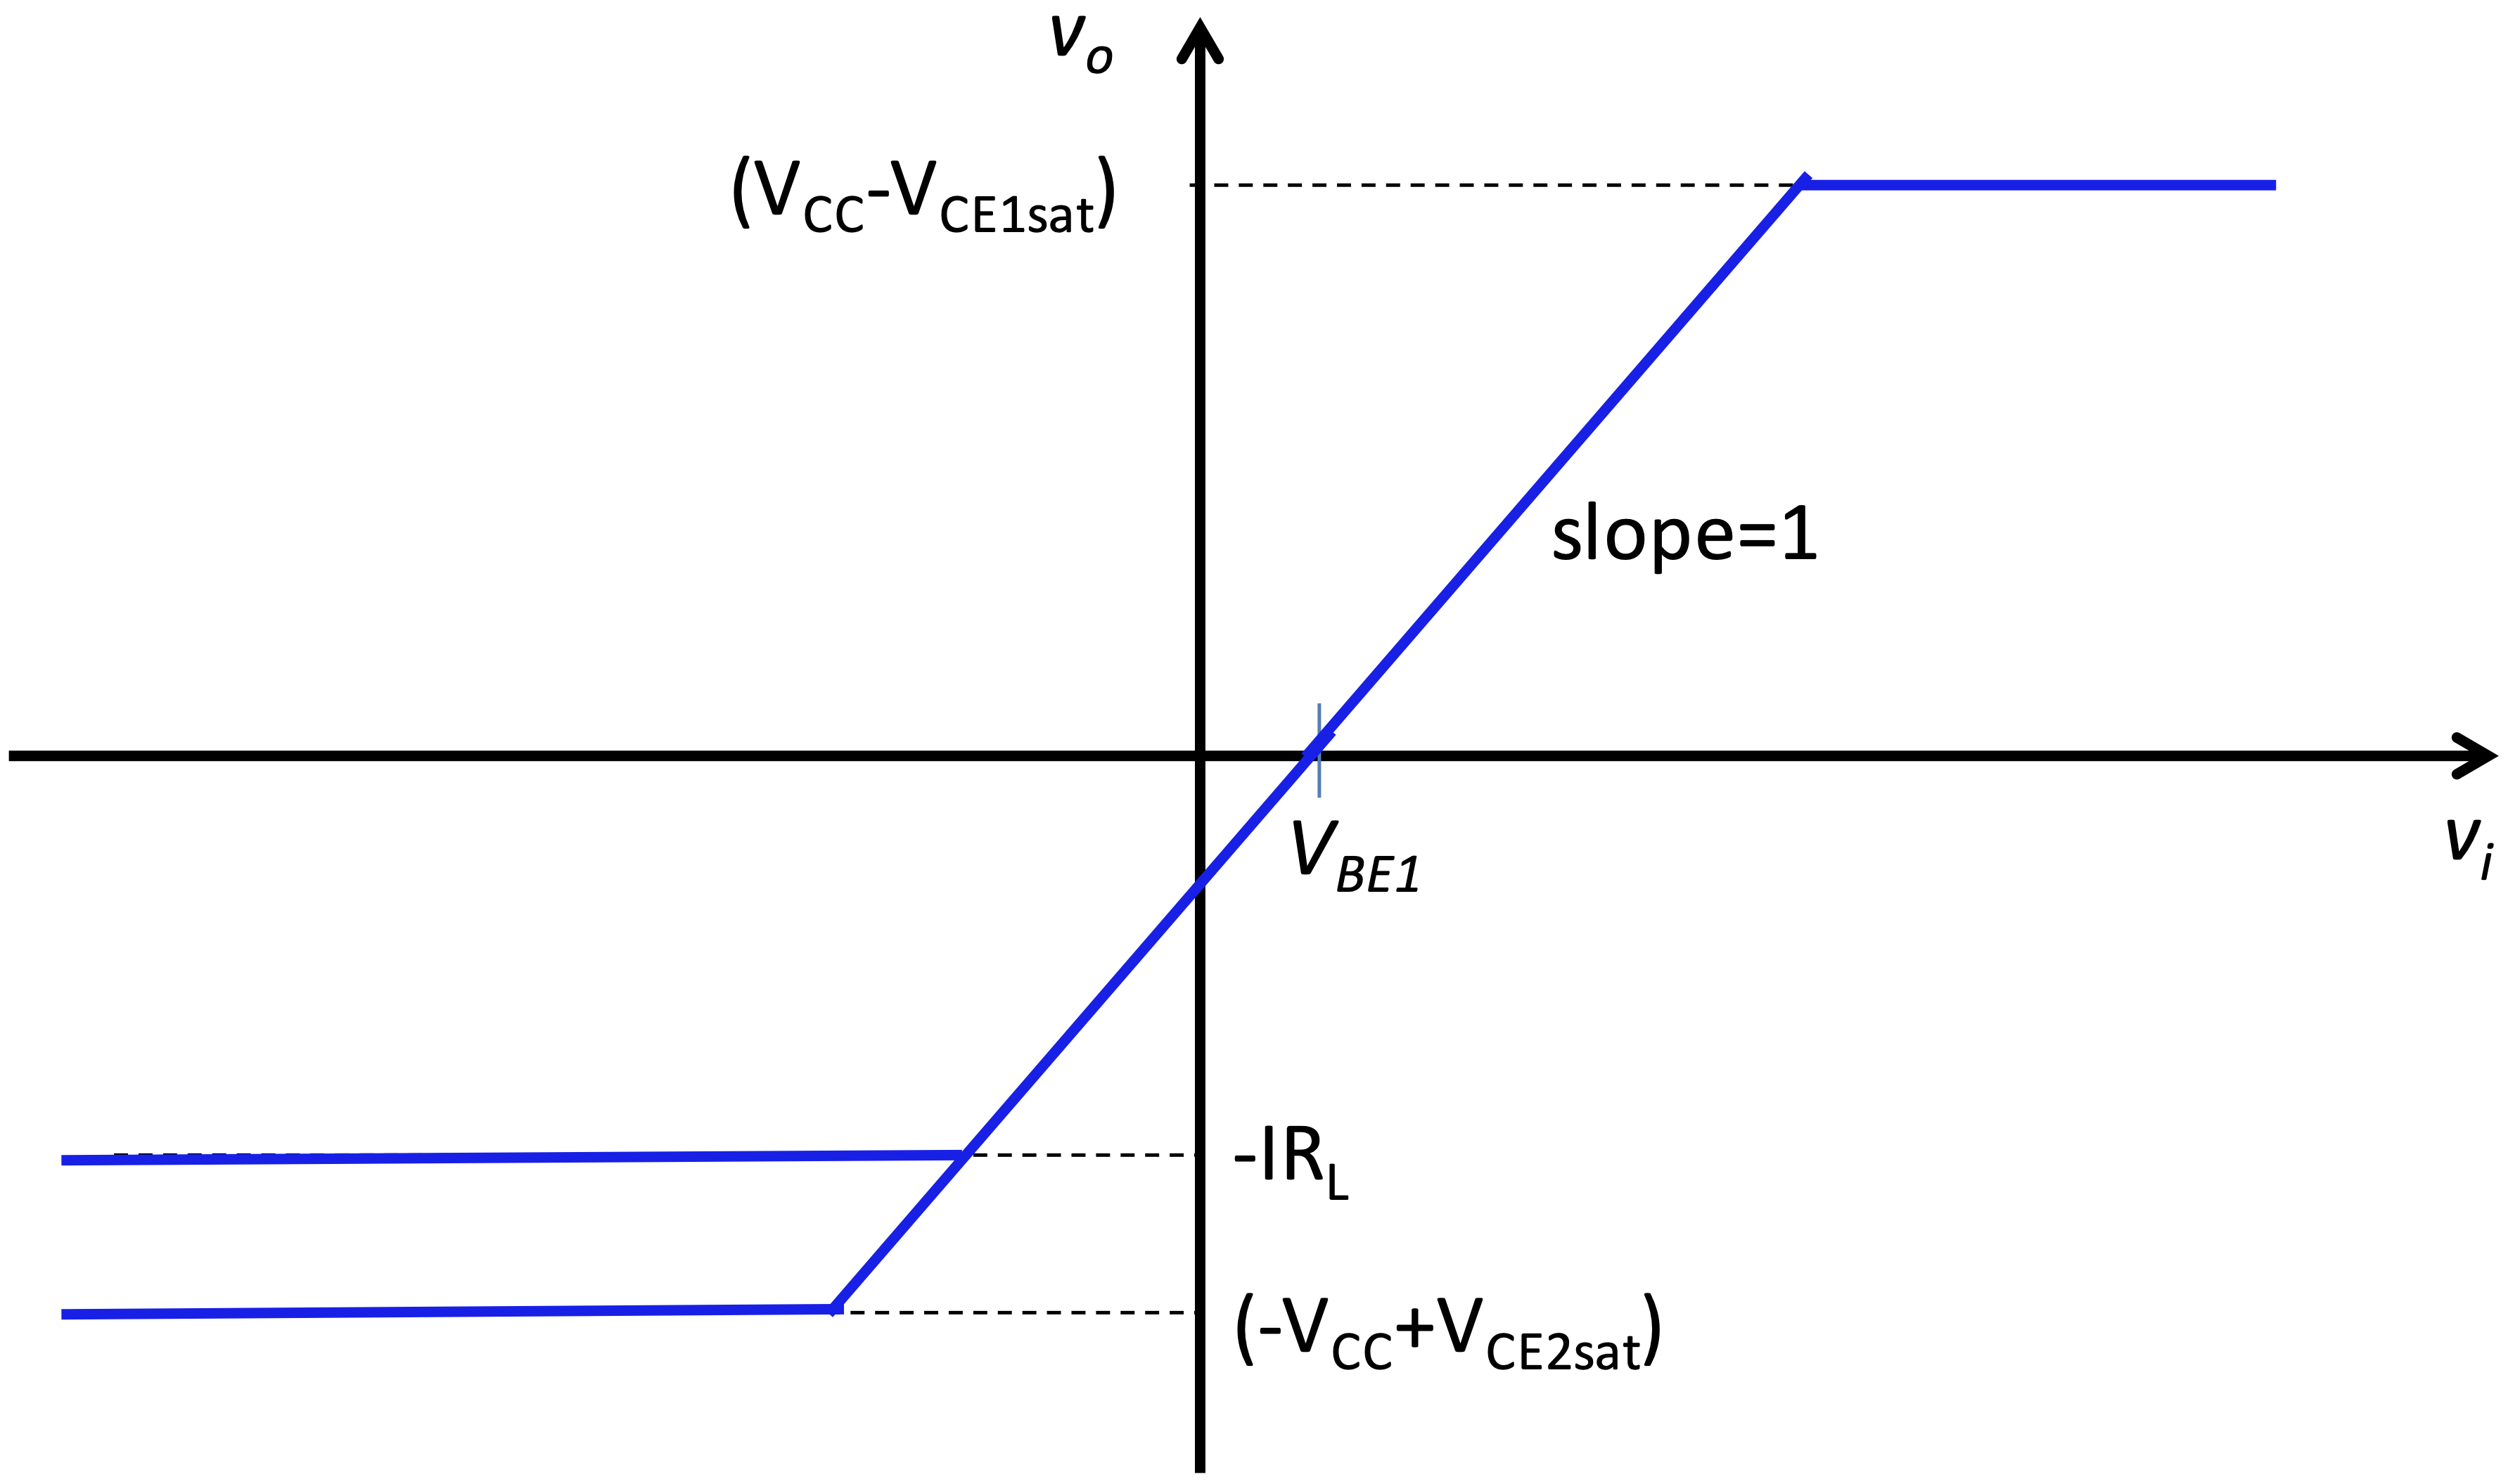
\includegraphics[width=\textwidth]{immagini/class_a_characteristic.png}
	\end{minipage}
	\begin{minipage}{0.5\textwidth}
		\begin{align*}
			V_{out} &= V_{in} - V_{BE1} \\
			& \\
			V_{out,max} &= V_{CC} - V_{CE1sat} \\
			V_{out,min} &= \max \left\{ -V_{CC} + V_{CE2sat}, \; -I_{gen} \cdot R_L \right\}
		\end{align*}
	\end{minipage}
\end{center}

\subsubsection*{Power dissipation}
In normal operation, when the load is connected and \(I_{gen} = V_{CC} / R_L\) (the maximum load current that absorb the load
when the output voltage is at its maximum), the maximum power dissipated by the transistor \(Q_1\) happens when the output voltage
is zero. This is the normal resting point of the output stage and it is one of the most common working points. The transistor
must be able to dissipate the power at this point for long periods of time without overheating.
\[V_{out} = 0 \; V \quad V_{CE1} = V_{CC} \quad I_{CE} = I_{gen} \quad \rightarrow \quad P_{Q_1, max} = V_{CC} \cdot I_{gen}\]
When the load is disconnected, the maximum power dissipated by \(Q_1\) happens when:
\[V_{out} = -V_{CC} \quad V_{CE1} = 2V_{CC} \quad I_{CE} = I_{gen} \quad \rightarrow \quad P_{Q_1, max, no-load} = 2 V_{CC} \cdot I_{gen}\]
When the load is short-circuited, the current through \(Q_1\) reach really high values (tends to infinity) and the \(Q_1\)
transistor can be destroyed by the high power dissipation. To prevent this, a short circuit protection can be implemented.

\subsubsection*{Power conversion efficiency}
The power conversion efficiency \(\eta\) of an output stage is defined as the ratio between the power delivered to the load
and the power drawn from the supply:
\[\eta = \frac{\text{load power } P_L}{\text{supply power } P_S}\]
For a class A output stage, the RMS power delivered to the load for a sinusoidal input signal is:
\[P_L = \frac{(V_{out}/\sqrt{2})^2}{R_L} = \frac{1}{2} \cdot \frac{{V_{out}}^2}{R_L}\]
The RMS power drawn from the supply is given by the sum of the power provided by the negative supply \(I_{gen} \cdot V_{CC}\)
and the power provided by the positive supply \((I_L + I_{gen}) \cdot V_{CC}\). For a sinusoidal input signal, the mean load
current is \(I_L = 0\), so the total power drawn from the supply is:
\[P_S = P_{S, negative} + P_{S, positive} = I_{gen} \cdot V_{CC} + (I_L + I_{gen}) \cdot V_{CC} = 2 I_{gen} \cdot V_{CC}\]
The power conversion efficiency of a class A output stage is therefore:
\[\eta = \frac{P_L}{P_S} = \frac{^1\!/_2 \cdot {V_{out}}^2 / R_L}{2 I_{gen} \cdot V_{CC}} = \frac{1}{4} \cdot \frac{V_{out}}{I_{gen} \cdot R_L} \frac{V_{out}}{V_{CC}} \leq 25\%\]
The maximum efficiency is achieved when \(V_{out} = V_{CC}\) and \(I_L = I_{gen} \rightarrow V_{out} = I_{gen} \cdot R_L\).

\subsubsection*{Advantages and disadvantages}
\begin{itemize}
	\item circuit is simple and easy to design, with really low distortion (THD \(\approx 0.1\%\))
	\item low efficiency (max 25\%) and high power dissipation makes it unsuitable for high power applications
	\item to avoid transistor saturation, output swing is limited and efficiency is even lower (10-20 \%)
\end{itemize}

\newpage

\subsection{Class B - Push-pull stage}
\subsubsection*{Circuit description}
The idea of the class B output stage is to use two complementary transistors \(Q_n\) and \(Q_p\) in a push-pull configuration:
one npn transistor drives the positive half of the input signal, while the other pnp transistor drives the negative half of
the input signal and only one transistor is on at a time.

\begin{center}
	\begin{circuitikz}[american, scale=0.8, transform shape]
		\node[npn, anchor=emitter] (Q1) at (0,0) {\(Q_n\)};
		\node[pnp, anchor=collector] (Q2) at (0,-2.5) {\(Q_p\)};
		\draw (Q1.B) -- ++(-0.7,0) -- node[midway] (input) {} ($(Q2.B) + (-0.7,0)$) -- (Q2.B);
		\draw ($(input)$) to[short, -o] ++(-0.7,0) node[left] {$V_{in}$};

		\draw (Q1.E) -- node[midway] (output) {} (Q2.E);
		\draw ($(output)$) to[short, -o, i_=\(I_L\)] ++(1.2,0) node[right] {$V_{out}$}
				to[R, l=\(R_L\)] ++(0, -2) ++(0,0.4)node[ground] {};

		\draw (Q1.C) to[short, -o] ++(0,0) node[above] {$+V_{CC}$};
		\draw (Q2.C) to[short, -o] ++(0,0) node[below] {\(-V_{CC}\)};
	
		\node [xshift=-0.1cm, yshift=-0.2cm] at (Q1.B) (vplus) {$+$};
		\node [xshift=-0.2cm, yshift=-0.2cm] at (Q1.E) (vminus) {$-$};
		\draw (vminus) to node[midway, fill=white, inner sep=3pt] {$V_{BEn}$} (vplus);

		\node [xshift=-0.2cm, yshift=0.2cm] at (Q2.E) (vplus) {$+$};
		\node [xshift=-0.1cm, yshift=0.2cm] at (Q2.B) (vminus) {$-$};
		\draw (vminus) to node[midway, fill=white, inner sep=3pt] {$V_{EBp}$} (vplus);
	\end{circuitikz}
\end{center}

\subsubsection*{Transfer characteristic}
The transfer characteristic of the class B output stage is a straight line with a slope of 1 with a dead zone called crossover
or ``notch'' distortion between \(-V_{EB,p}\) and \(V_{BE,n}\).

\begin{center}
	\begin{minipage}{0.45\textwidth}
		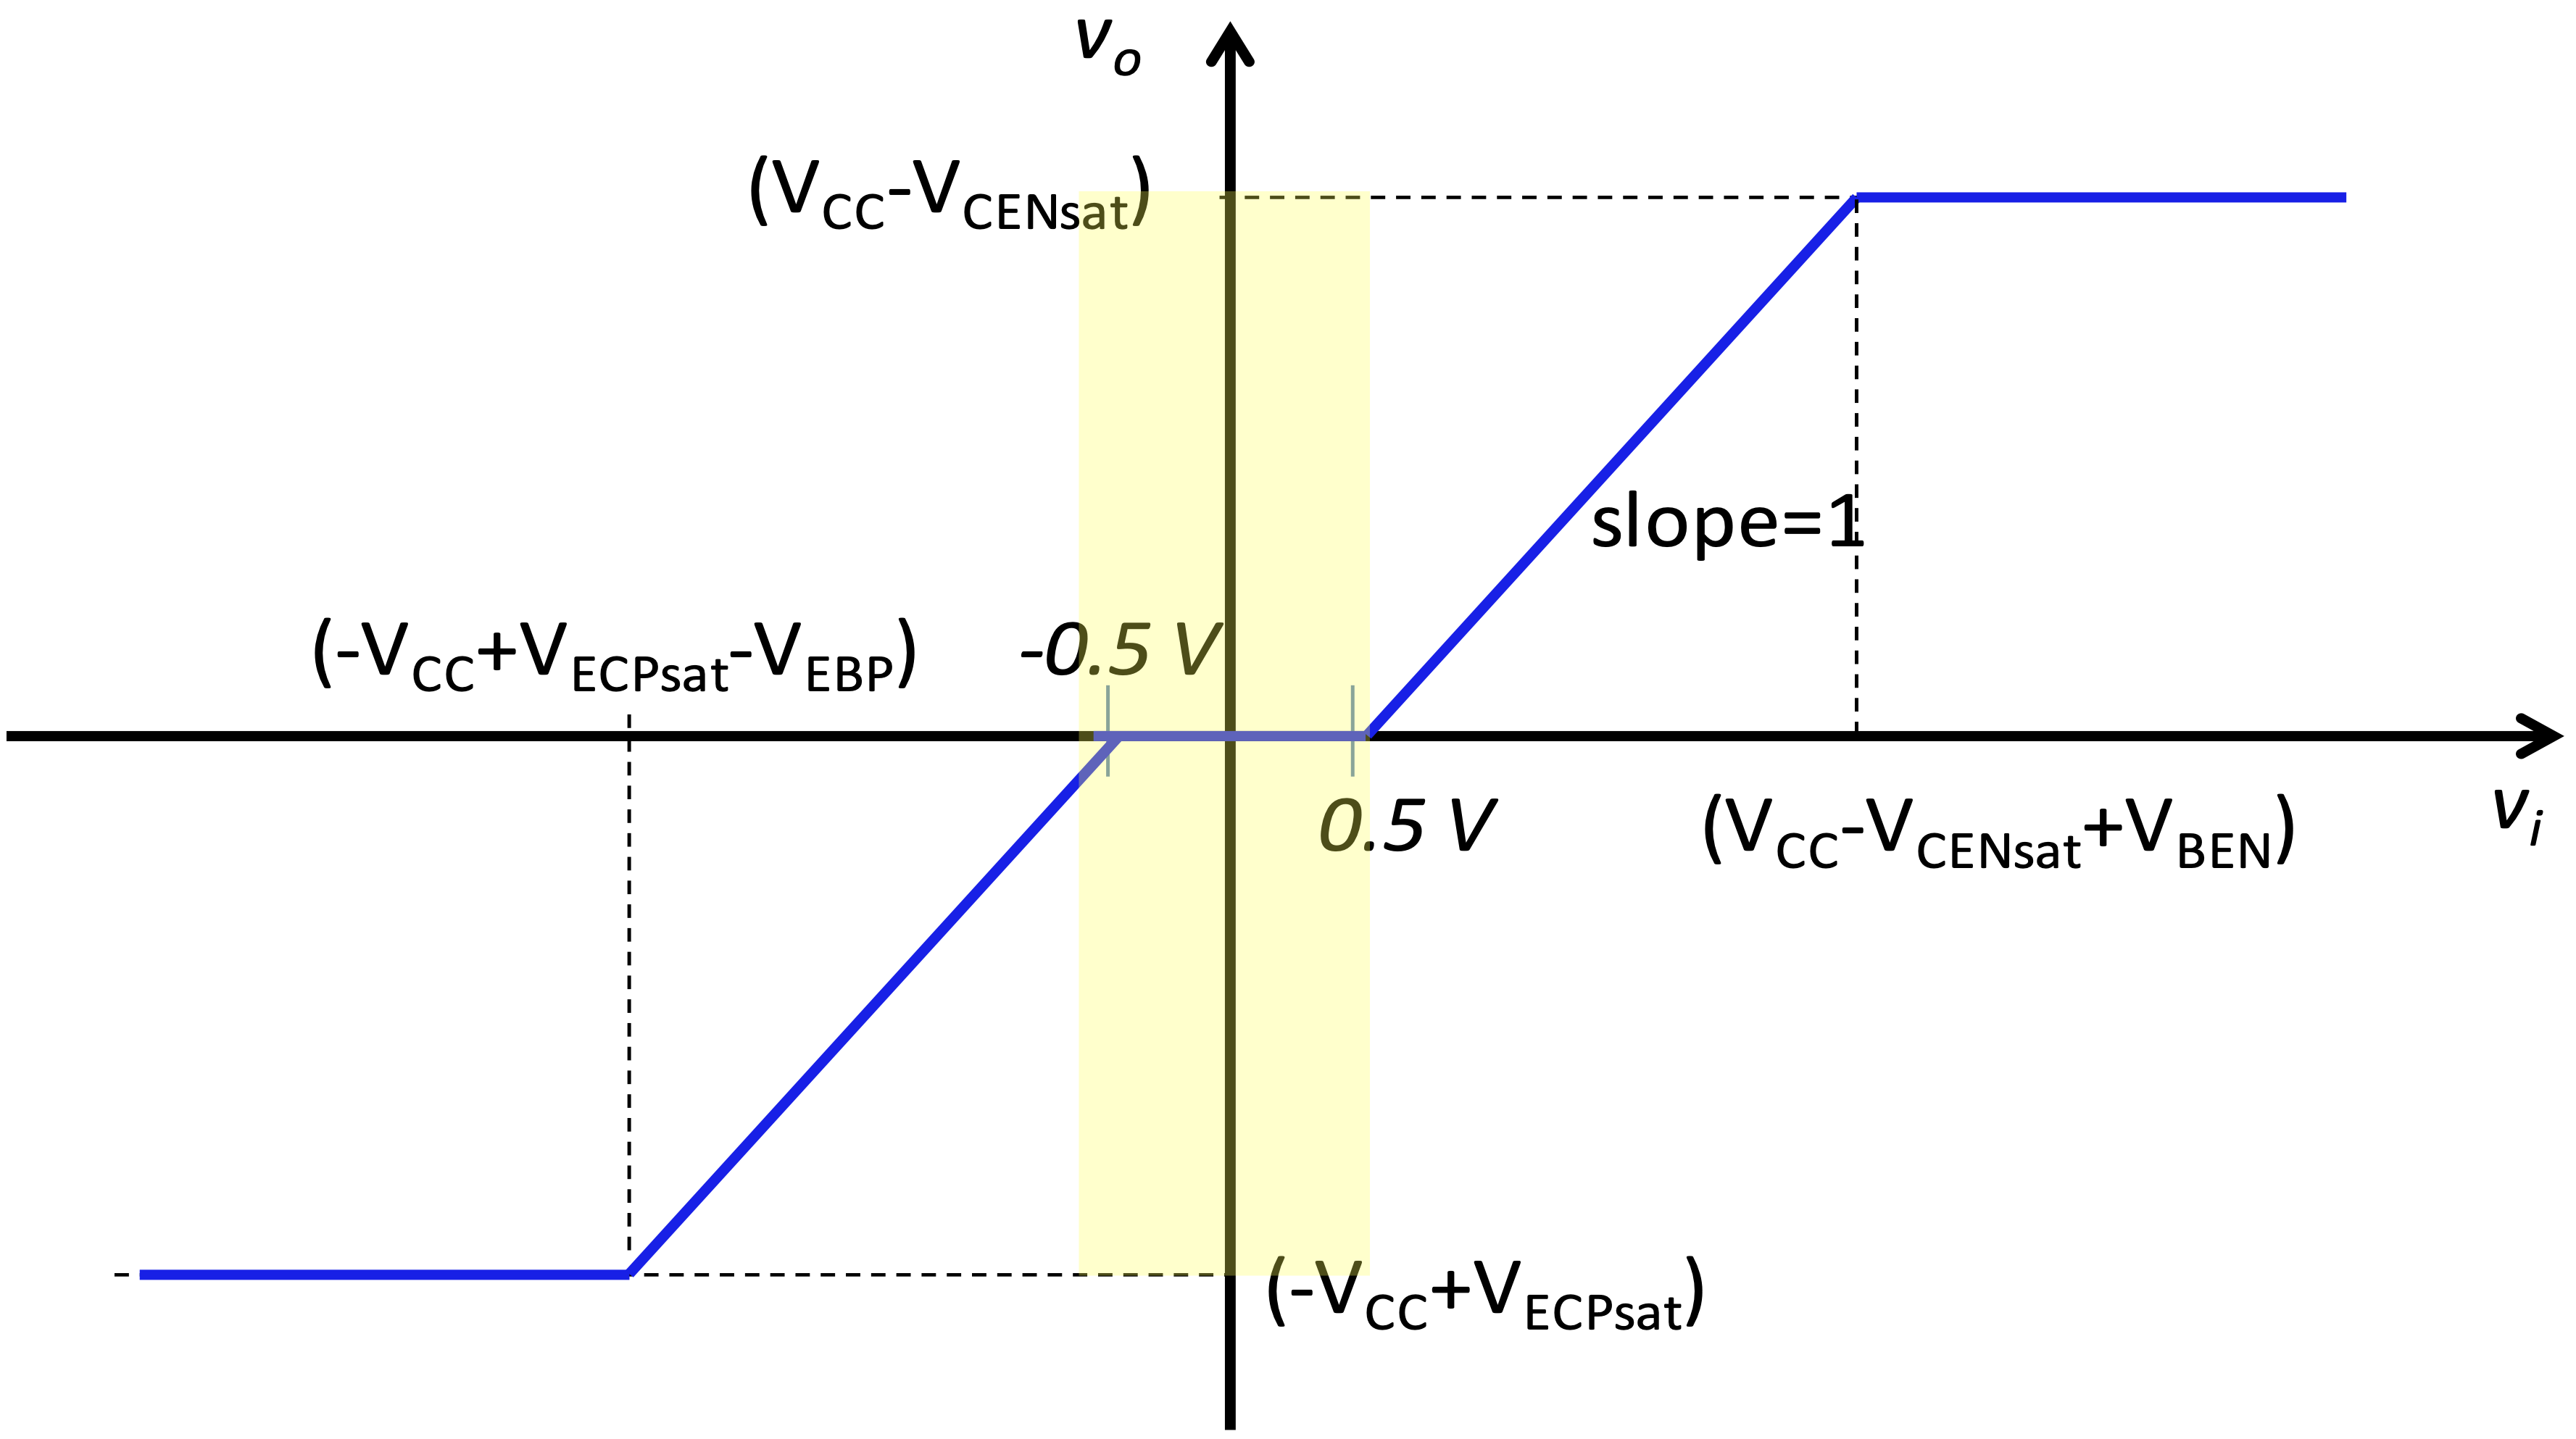
\includegraphics[width=\textwidth]{immagini/class_b_characteristic.png} \\[0.5cm]
		\footnotesize Transfer characteristic of a class B output stage
	\end{minipage}
	\begin{minipage}{0.5\textwidth}
		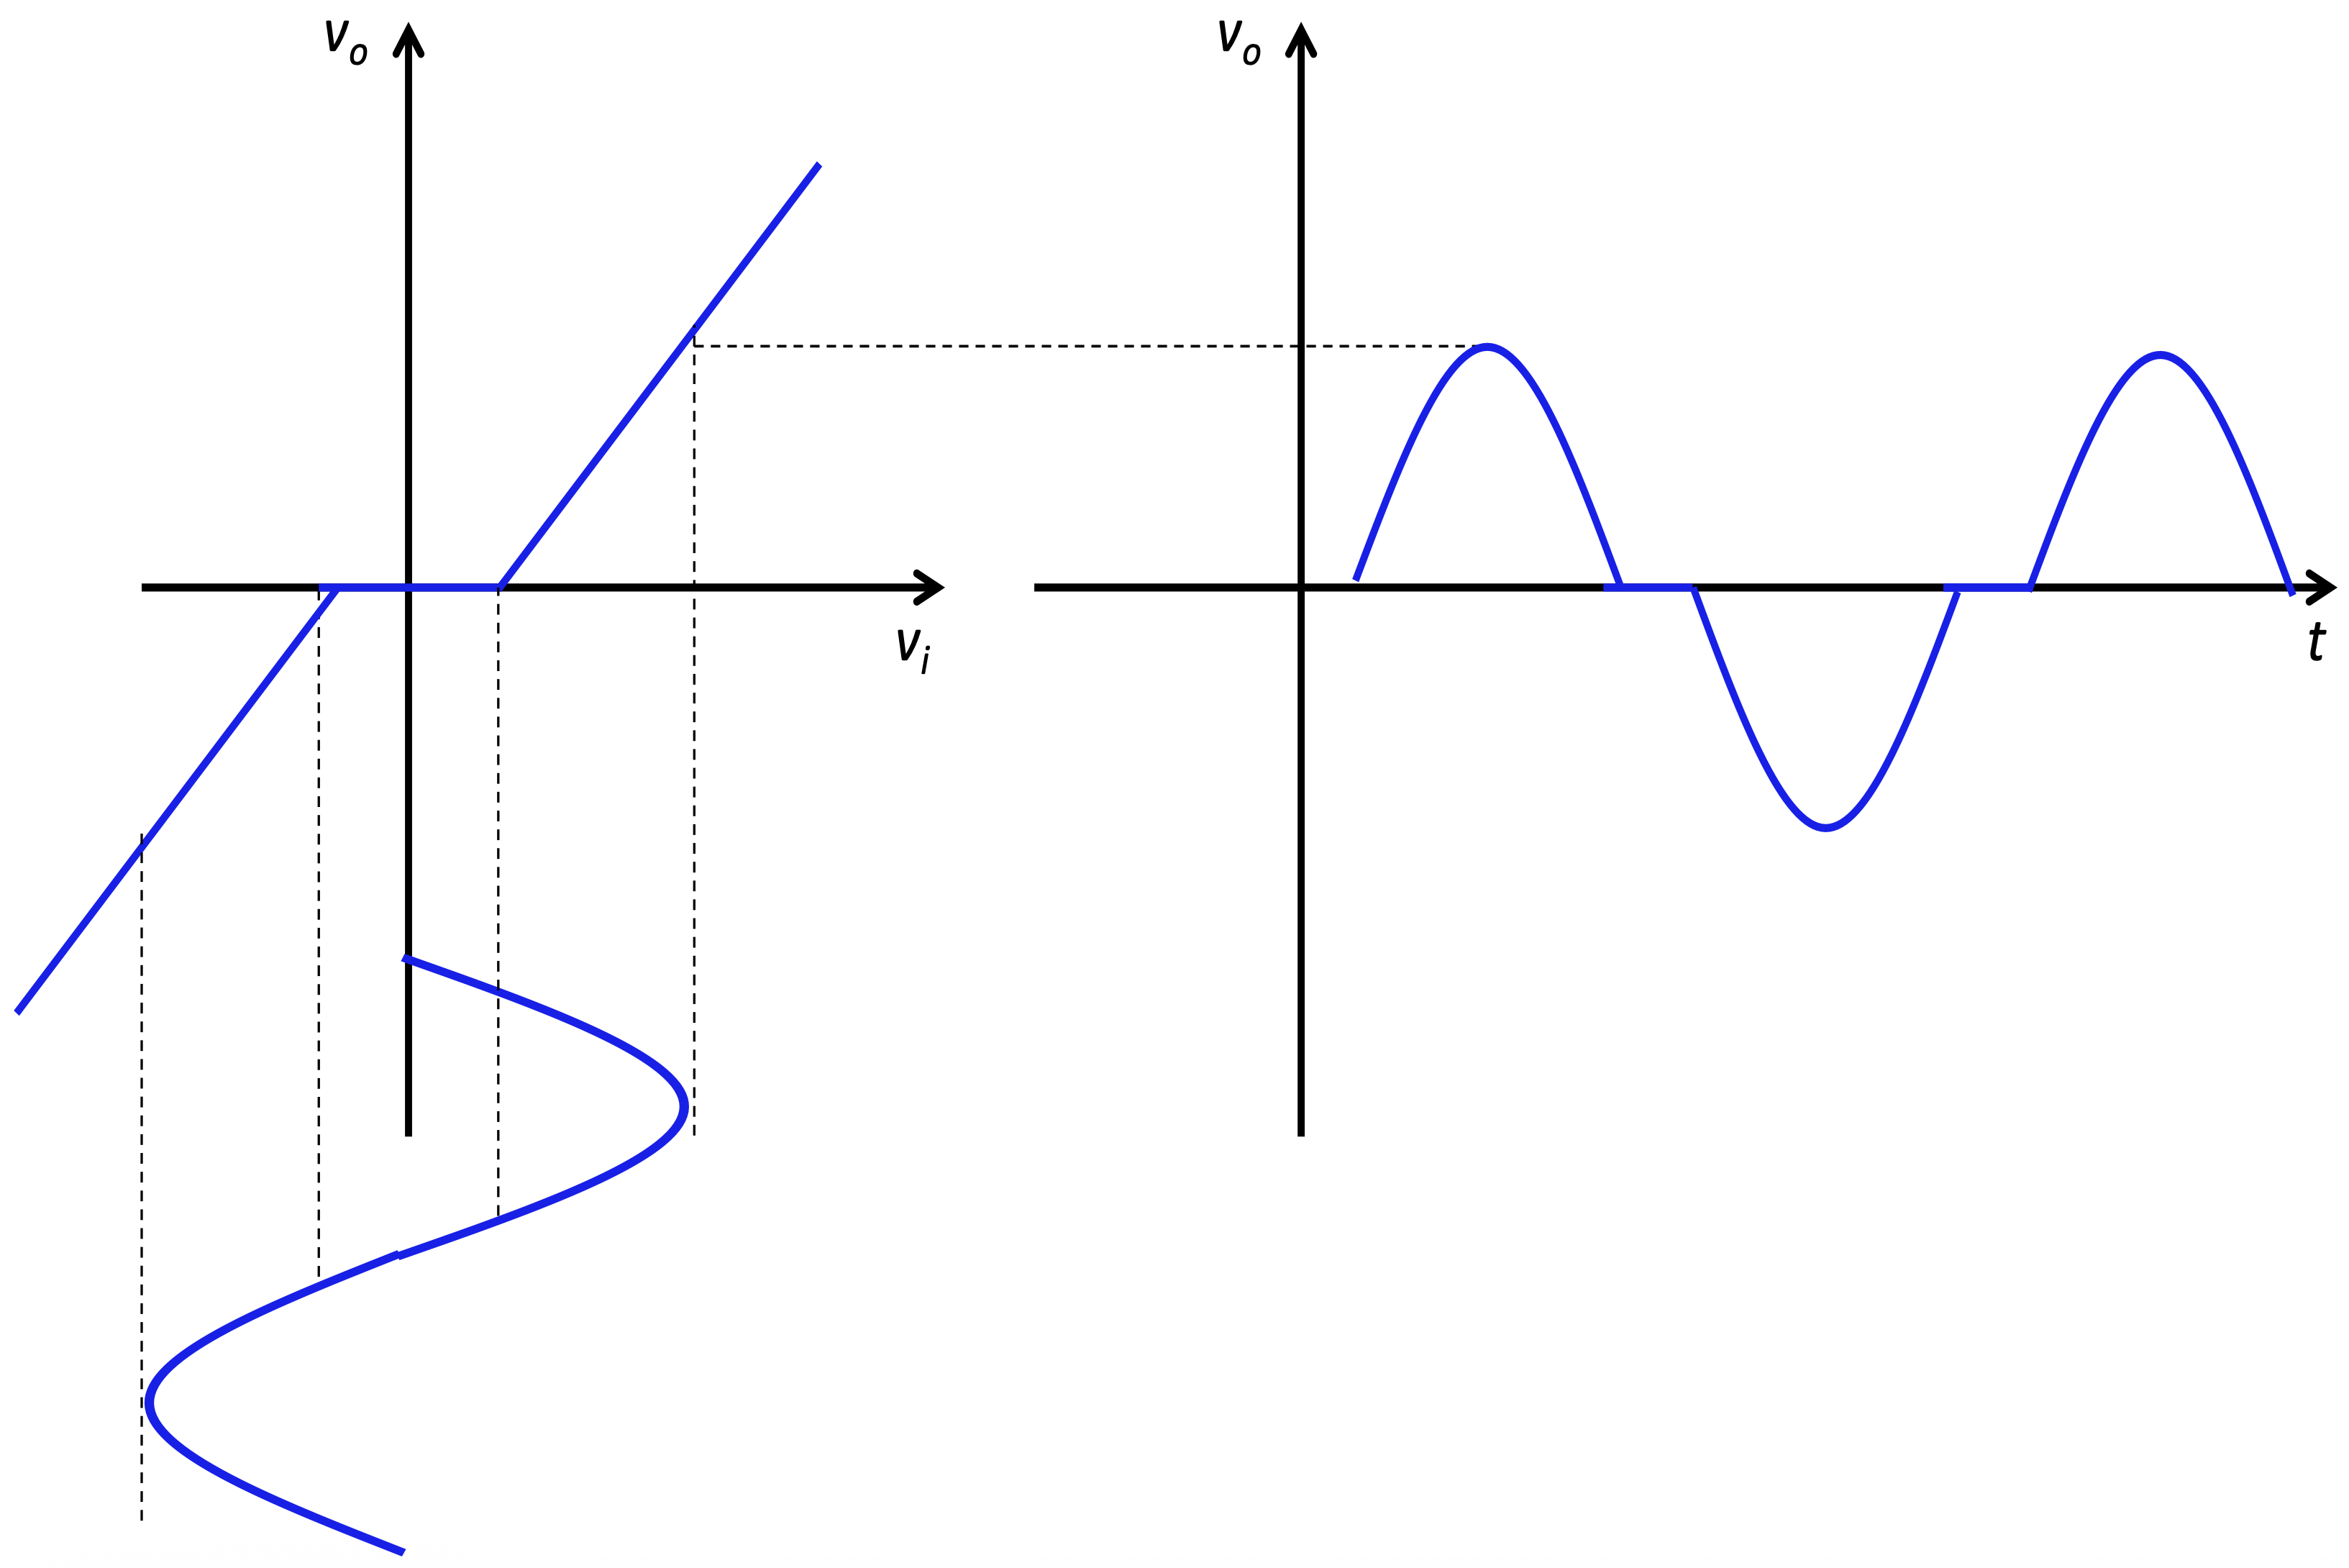
\includegraphics[width=0.8\textwidth]{immagini/class_b_curve.png} \\[0.5cm]
		\footnotesize Example of input and output signals (sinusoidal) of a class B output stage, the crossover distortion is
		clearly visible around the zero crossing of the output signal.
	\end{minipage}
\end{center}

\subsubsection*{Power conversion efficiency}
Can be demonstrated that the maximum power conversion efficiency of a class B output stage is:
\[\eta_{max} = \frac{\pi}{4} = 78.5\%\]

\subsubsection*{Crossover distortion}
The crossover distortion is the distortion that occurs in the output signal when the input signal is around zero, due to the dead
zone between \(-V_{EB,p}\) and \(V_{BE,n}\).

\vspace{10pt}

\begin{center}
	\begin{minipage}{0.5\textwidth}
		\begin{circuitikz}[american, scale=0.8, transform shape]
			\node[npn, anchor=emitter] (Q1) at (0,0) {\(Q_n\)};
			\node[pnp, anchor=collector] (Q2) at (0,-2.5) {\(Q_p\)};
			\draw (Q1.B) -- ++(-0.7,0) -- node[midway] (input) {} ($(Q2.B) + (-0.7,0)$) -- (Q2.B);
	
			\draw (Q1.E) -- node[midway] (output) {} (Q2.E);
			\draw ($(output)$) to[short, -o, i_=\(I_L\), current/distance=0.3] ++(1.5,0) node[right] {$V_{out}$}
				to[R, l=\(R_L\)] ++(0, -2) ++(0,0.4)node[ground] {};
	
			\draw (Q1.C) to[short, -o] ++(0,0) node[above] {$+V_{CC}$};
			\draw (Q2.C) to[short, -o] ++(0,0) node[below] {\(-V_{CC}\)};
		
			\node [xshift=-0.1cm, yshift=-0.2cm] at (Q1.B) (vplus) {$+$};
			\node [xshift=-0.2cm, yshift=-0.2cm] at (Q1.E) (vminus) {$-$};
			\draw (vminus) to node[midway, fill=white, inner sep=3pt] {$V_{BEn}$} (vplus);
	
			\node [xshift=-0.2cm, yshift=0.2cm] at (Q2.E) (vplus) {$+$};
			\node [xshift=-0.1cm, yshift=0.2cm] at (Q2.B) (vminus) {$-$};
			\draw (vminus) to node[midway, fill=white, inner sep=3pt] {$V_{EBp}$} (vplus);
	
			\node[op amp, anchor=out] (opamp) at ($(input) + (-0.5,0)$) {};
			\draw (opamp.out) -- ($(input)$);
			\draw (opamp.+) to[short, -o] ++(-0.5,0) node[left] {$V_{in}$};
			\draw (opamp.-) -- ++(-0.5, 0) -- ++(0,2.1) -- ++(5.62,0) -- ($(output) + (0.7,0)$) node[circ] {};
		\end{circuitikz}
	\end{minipage}
	\begin{minipage}{0.45\textwidth}
		This distortion can be reduced by using an op amp to drive the input signal of the output stage with feedback loop
		to compensate the dead zone as shown on the left.

		\vspace{10pt}
		
		It is important to keep in mind op amps limitations, especially low slew rates can limit the compensation.
	\end{minipage}
\end{center}

\newpage

\subsection{Class AB}
\subsubsection*{Circuit description}
The main idea of the class AB output stage is to reuse the same push-pull configuration of the class B output stage, but with
a bias voltage \(V_{BB}\) applied to the bases of both transistors \(Q_n\) and \(Q_p\) to keep them slightly on even without
input signal. In this way, transistors are always slightly conductive and are able to drive immediately the output signal
without the class B delay and the crossover distortion is virtually eliminated.

\begin{center}
	\begin{minipage}{0.45\textwidth}
		\centering \begin{circuitikz}[american, scale=0.8, transform shape]
			\node[npn, anchor=emitter] (Q1) at (0,0) {\(Q_n\)};
			\node[pnp, anchor=collector] (Q2) at (0,-3) {\(Q_p\)};
			\draw (Q1.B) -- ++(-2.4,0);
			\draw (Q2.B) -- ++(-2.4,0);
			\draw ($(Q1.B)+(-2.4,0)$) to[battery1, v=\(V_{BB}/2\)] ($($(Q2.B) + (-2.4,0)$)!0.5!($(Q1.B) + (-2.4,0)$)$) node (input) {} to[battery1, v=\(V_{BB}/2\)] ($(Q2.B)+(-2.4,0)$);
			\draw ($(input)$) to[short, -o] ++(-1,0) node[left] {$V_{in}$};
	
			\draw (Q1.E) to[short, i=\(I_{N}\)] ($($(Q2.E)!0.5!(Q1.E)$) + (0,0.2)$) -- ++(0,-0.2) node (output) {} -- ++(0,-0.2) to[short, i=\(I_{P}\)] (Q2.E);
			
			\draw ($(output)$) -- ++(0.5,0) to[short, -o, i=\(I_L\)] ++(1.2,0) node[right] {$V_{out}$}
				to[R, l=\(R_L\)] ++(0, -2) ++(0,0.4)node[ground] {};
	
			\draw (Q1.C) to[short, -o] ++(0,0) node[above] {$+V_{CC}$};
			\draw (Q2.C) to[short, -o] ++(0,0) node[below] {\(-V_{CC}\)};
	
			\node [xshift=-0.1cm, yshift=-0.2cm] at (Q1.B) (vplus) {$+$};
			\node [xshift=-0.3cm, yshift=-0.1cm] at (Q1.E) (vminus) {$-$};
			\draw (vminus) to node[midway, fill=white, inner sep=3pt] {$V_{BEn}$} (vplus);
	
			\node [xshift=-0.3cm, yshift=0.1cm] at (Q2.E) (vplus) {$+$};
			\node [xshift=-0.1cm, yshift=0.2cm] at (Q2.B) (vminus) {$-$};
			\draw (vminus) to node[midway, fill=white, inner sep=1pt] {$V_{EBp}$} (vplus);
		\end{circuitikz} \\[0.5cm]
		\footnotesize Circuit of a class AB output stage with bias voltage \(V_{BB}\) applied via two ideal voltage sources.
	\end{minipage}
	\begin{minipage}{0.45\textwidth}
		\centering \begin{circuitikz}[american, scale=0.8, transform shape]
			\ctikzset{diodes/scale=0.8, capacitors/scale=0.8, resistors/scale=0.8}
			
			\node[npn, anchor=emitter] (Q1) at (0,0) {\(Q_n\)};
			\node[pnp, anchor=collector] (Q2) at (0,-3) {\(Q_p\)};
			
			\draw (Q1.C) to[short, -o] ++(0,1) node (vcc) {} node[above] {$+V_{CC}$};
			\draw (Q2.C) to[short, -o] ++(0,-1) node (vss) {}node[below] {\(-V_{CC}\)};

			\draw (Q1.B) -- ++(-1,0) node (base11) {} to[C, l=\(C_1\)] ++(-1.5,0) node (base12) {};
			\draw (Q2.B) -- ++(-1,0) node (base21) {} to[C, l=\(C_2\)] ++(-1.5,0) node (base22) {};
			\draw ($(base11)$) to[D] ($(base11)!0.5!(base21)$) to[D] ($(base21)$);
			\draw ($(base12)$) -- ($(base12)!0.5!(base22)$) node (input) {} -- ($(base22)$);
			\draw ($(base11)$) to[R, l_=\(R_1\)] ++(0.5,+1.5) -| (vcc);
			\draw ($(base21)$) to[R, l=\(R_2\)] ++(0.5,-1.5) -| (vss);
			\draw ($(input)$) to[short, -o] ++(-1,0) node[left] {$V_{in}$};
	
			\draw (Q1.E) to[short, i=\(I_{N}\)] ($($(Q2.E)!0.5!(Q1.E)$) + (0,0.2)$) -- ++(0,-0.2) node (output) {} -- ++(0,-0.2) to[short, i=\(I_{P}\)] (Q2.E);
			
			\draw ($(output)$) -- ++(0.5,0) to[short, -o, i=\(I_L\)] ++(1.2,0) node[right] {$V_{out}$}
				to[R, l=\(R_L\)] ++(0, -2) ++(0,0.4)node[ground] {};
	
			\node [xshift=-0.1cm, yshift=-0.2cm] at (Q1.B) (vplus) {$+$};
			\node [xshift=-0.3cm, yshift=-0.1cm] at (Q1.E) (vminus) {$-$};
			\draw (vminus) to node[midway, fill=white, inner sep=3pt] {$V_{BEn}$} (vplus);
	
			\node [xshift=-0.3cm, yshift=0.1cm] at (Q2.E) (vplus) {$+$};
			\node [xshift=-0.1cm, yshift=0.2cm] at (Q2.B) (vminus) {$-$};
			\draw (vminus) to node[midway, fill=white, inner sep=1pt] {$V_{EBp}$} (vplus);
		\end{circuitikz} \\[0.5cm]
		\footnotesize Circuit of a class AB output stage with bias voltage \(V_{BB}\) applied via two diodes.
	\end{minipage}
\end{center}

In real circuits, the bias voltage \(V_{BB}\) is imposed by using two diodes connected in series between the bases of the
two transistors \(Q_n\) and \(Q_p\) as shown on the right. There are also two capacitors \(C_1\) and \(C_2\) to filter the
bias voltage and two resistors \(R_1\) and \(R_2\) to properly limit the current through the diodes. 

\subsubsection*{Circuit behavior}
\begin{itemize}
	\item[1.] When the input signal passes from zero to positive, the \(Q_n\) transistor starts to conduct more current
	and \(V_{BEn}\) increases. Due to the fact that \(V_{BEn} + V_{EBp} = V_{BB}\), the \(V_{EBp}\) decreases and the
	\(Q_p\) transistor starts to conduct less current until it reaches its minimum conduction.
	\item[2.] Vice versa, when the input signal passes from zero to negative, the \(Q_p\) transistor starts to conduct more
	current and \(V_{EBp}\) increases. The \(V_{BEn}\) decreases and the \(Q_n\) transistor starts to conduct less current
	until it reaches its minimum conduction.
\end{itemize}

If the bias voltage \(V_{BB}\) is big enough, both transistors are slightly conductive at zero input signal and are able
to immediately drive the output signal without delay eliminating the crossover distortion. If the bias voltage \(V_{BB}\)
is too big, it is possible that both transistors remain conductive for the entire input signal period, and the output stage
behaves like a class A output stage with high power dissipation and low efficiency.

\subsubsection*{Quiescent power dissipation}
The problem of this configuration is that when both transistors are on at the same time, there is a direct current flowing from
the positive supply to the negative supply through the transistors, that increases power dissipation and reduces efficiency.

If the \(V_{BB}\) is properly chosen, the quiescent current \(I_{Q}\) is smaller than the load current \(I_L\), so the quiescent
power dissipation is negligible and the efficiency is close to the maximum efficiency of a class B output stage.

\subsubsection*{Current analysis}
From the diode equations applied to the npn and pnp transistors:
\begin{align*}
	I_{N} &= I_S \left( e^{V_{BEn} / V_T} - 1 \right) \approx I_S \left( e^{V_{BEn} / V_T} \right) \quad \rightarrow \quad V_{BEn} = V_T \ln \left( \frac{I_N}{I_S} \right) \\
	I_{P} &= I_S \left( e^{V_{EBp} / V_T} - 1 \right) \approx I_S \left( e^{V_{EBp} / V_T} \right)\quad \rightarrow \quad V_{EBp} = V_T \ln \left( \frac{I_P}{I_S} \right) \\
	I_{Q} &= I_S \left( e^{V_{BB} / 2 V_T} - 1 \right) \approx I_S \left( e^{V_{BB} / 2 V_T} \right) \quad \rightarrow \quad V_{BB} = 2 V_T \ln \left( \frac{I_Q}{I_S} \right)
\end{align*}
\[V_{BEn} + V_{EBp} = V_{BB} \quad \rightarrow \quad V_T \ln \left( \frac{I_N}{I_S} \right) + V_T \ln \left( \frac{I_P}{I_S} \right) = 2 V_T \ln \left( \frac{I_Q}{I_S} \right) \quad \rightarrow \quad I_N \cdot I_P = {I_Q}^2\]

From the Kirchhoff's current law at the output node: \[I_N = I_P + I_L\]

Putting both equations together: \[I_N^2 - I_L \cdot I_N - I_Q^2 = 0\]

By solving the quadratic equation, we can find the current \(I_N\) and \(I_P\):
\[I_N = \frac{I_L}{2} + \sqrt{\left(\frac{I_L}{2}\right)^2 + I_Q^2} \qquad I_P = -\frac{I_L}{2} + \sqrt{\left(\frac{I_L}{2}\right)^2 + I_Q^2}\]
These results show that:
\begin{itemize}
	\item if \(I_L = 0\), then \(I_N = I_P = I_Q\) and both transistors are slightly conductive
	\item if \(I_L\) is big enough, then \(I_N \approx I_L\) and \(I_P \approx 0\) (or vice versa if \(I_L\) is negative), by
	neglecting the \({I_Q}^2\) term in the square root, showing that the output stage behaves like a class B output stage when
	the load current is big enough
\end{itemize}

\subsubsection*{Transfer characteristic}
The transfer characteristic of the class AB output stage with ideal bias voltage \(V_{BB}\) is a perfect straight line with a
slope of 1, no crossover distortion and no voltage offset.
\begin{center}
	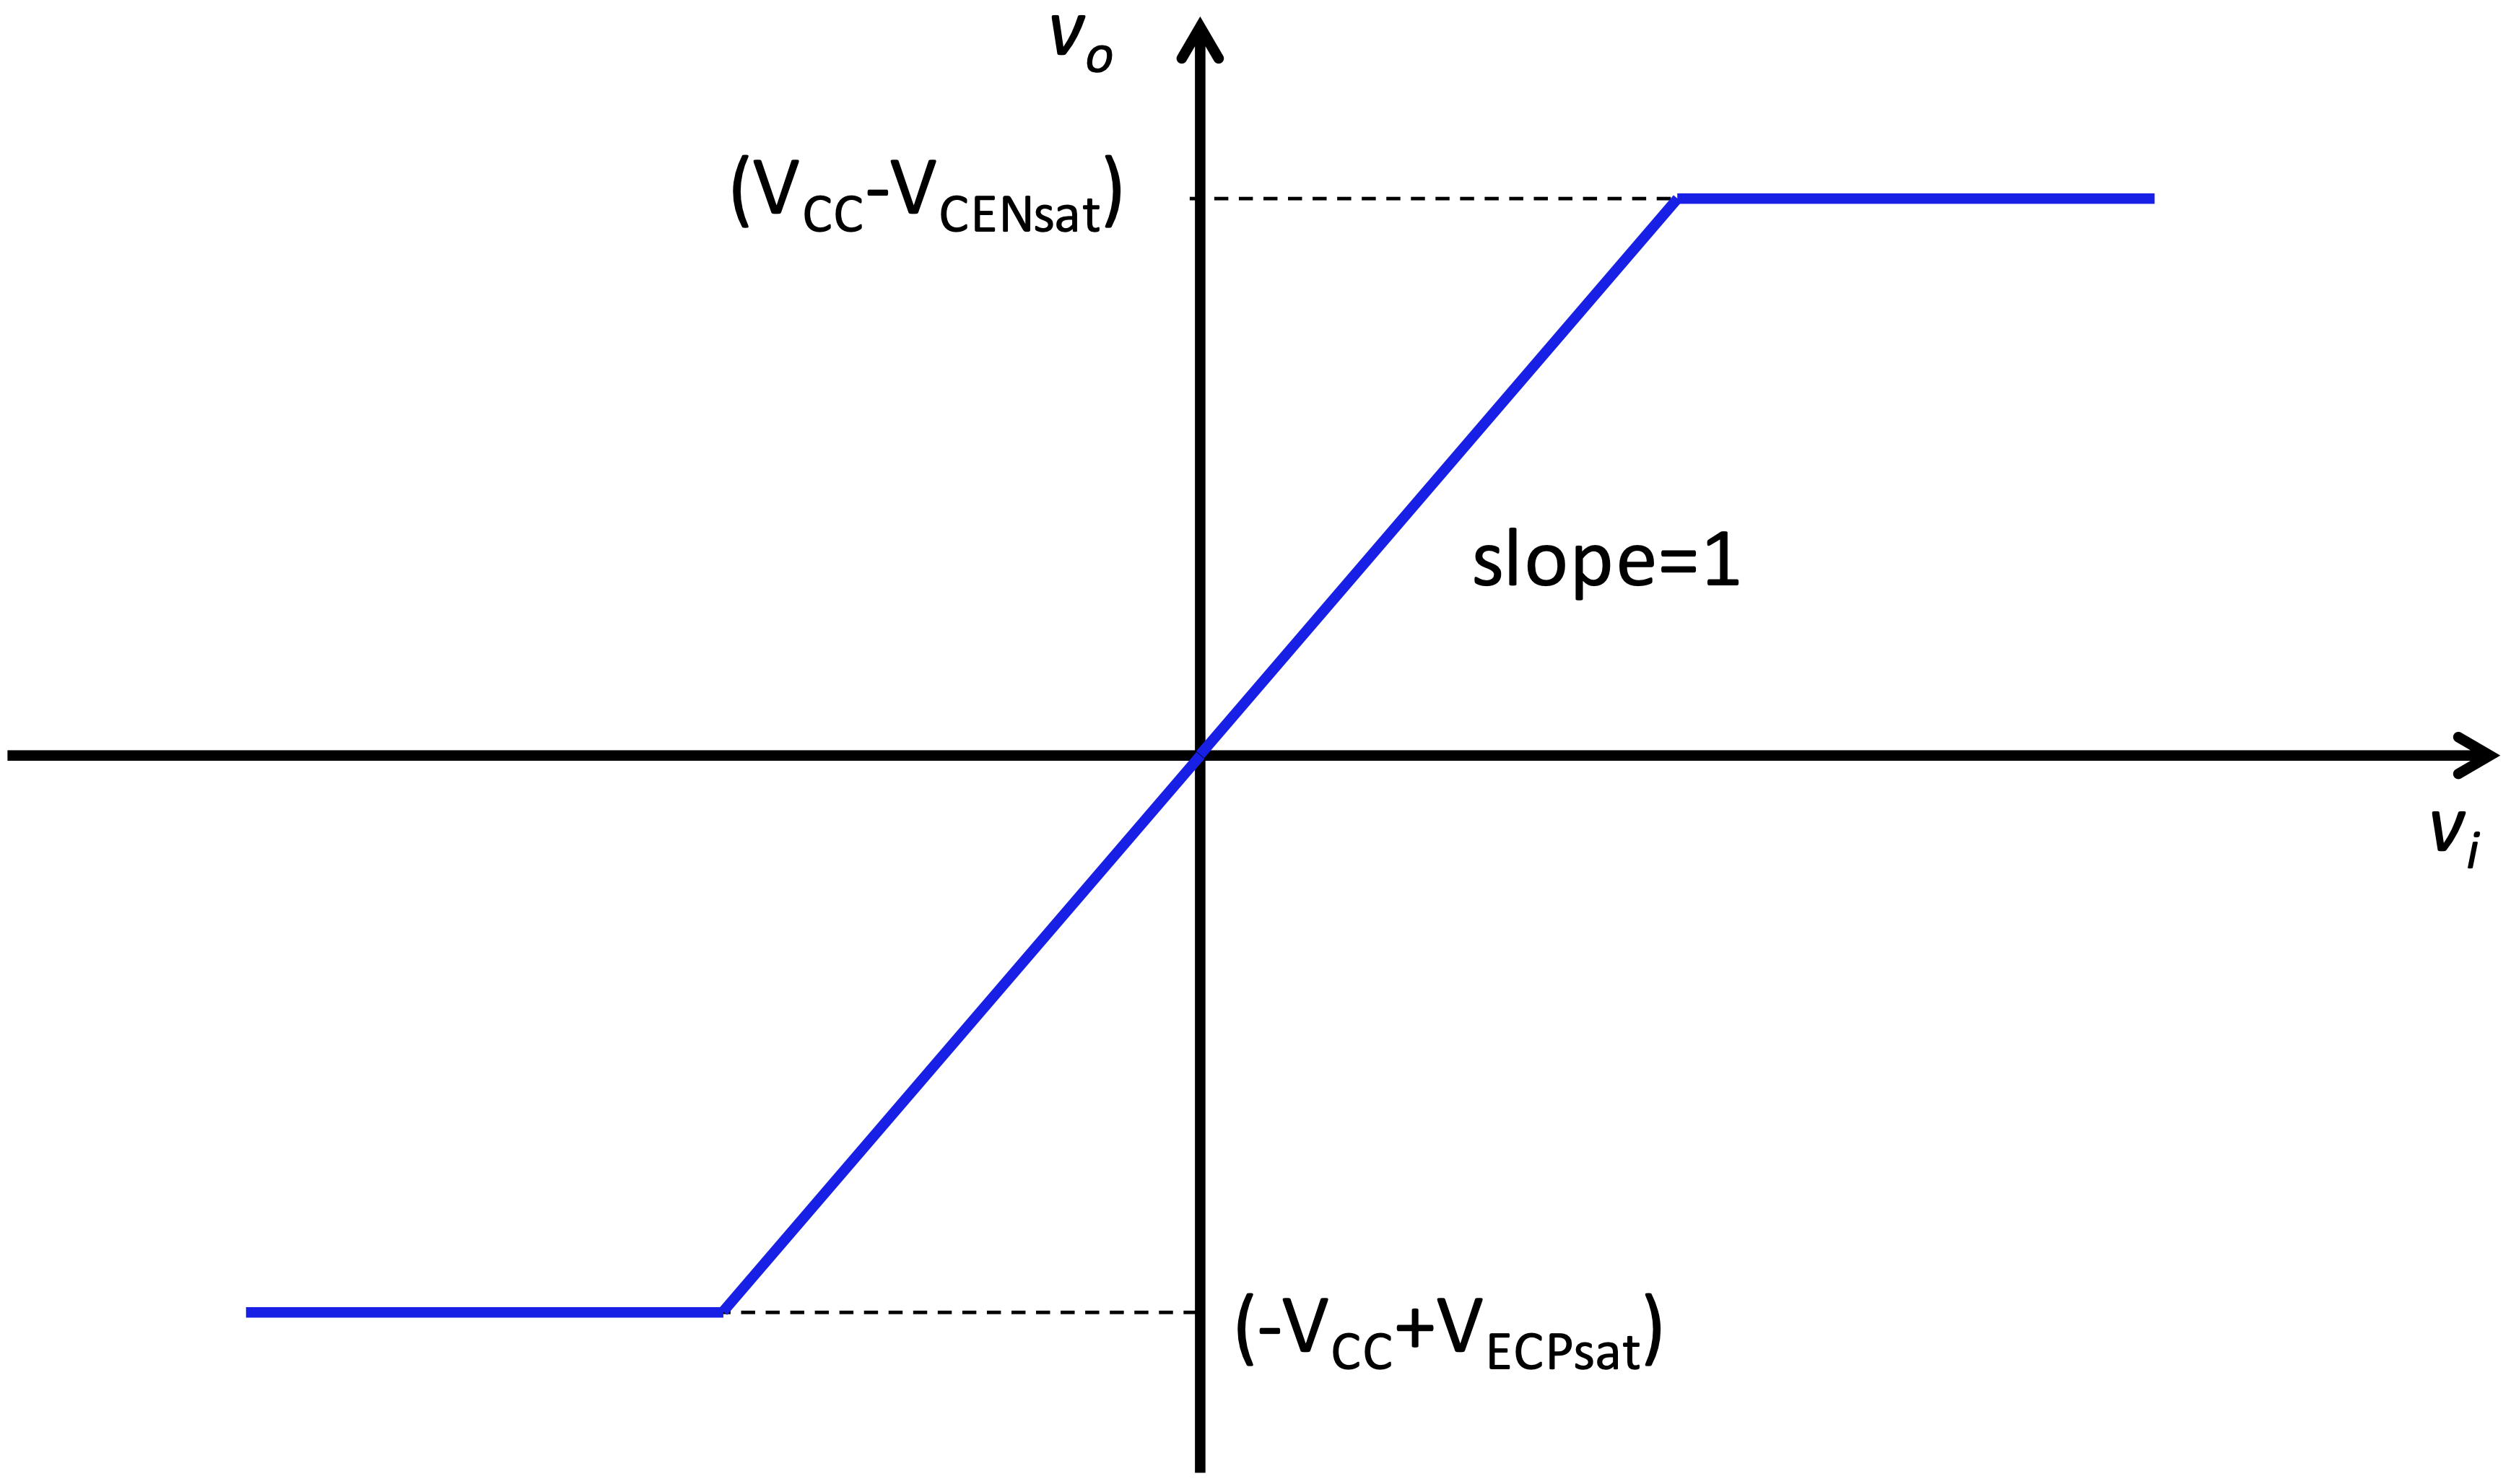
\includegraphics[width=0.5\textwidth]{immagini/class_ab_characteristic.png}
\end{center}

\subsubsection*{Disadvantages}
The main problem of the class AB output stage is to properly set the bias voltage \(V_{BB}\) to eliminate crossover distortion
without increasing too much the quiescent power dissipation. This is a really hard task in real circuits because of the
components tolerances and the temperature variations.
